\subsection{正多面体}\label{subsec:3-3}
\begin{enhancedline}

常见的食盐的结晶(图 \ref{fig:ltjh-3-7})、明矾的结晶(图 \ref{fig:ltjh-3-8})都呈正多面体的形状。

\begin{figure}[htbp]
    \centering
    \begin{minipage}[b]{5cm}
        \centering
        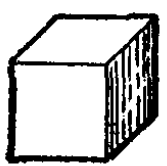
\includegraphics[width=2cm]{../pic/ltjh-ch3-07.png}
        \caption{}\label{fig:ltjh-3-7}
    \end{minipage}
    \qquad \qquad
    \begin{minipage}[b]{5cm}
        \centering
        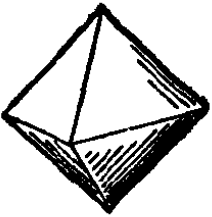
\includegraphics[width=2cm]{../pic/ltjh-ch3-08.png}
        \caption{}\label{fig:ltjh-3-8}
    \end{minipage}
\end{figure}

每个面都是有同数边的正多边形,在每个顶点都有同数棱的凸多面体,叫做\zhongdian{正多面体}。
例如,正方体的所有面都是正方形,在各个顶点都有三条棱,而且是凸多面体,所以正方体就是一种正多面体。

我们知道,正多边形有无限多种,那么正多面体能有多少种呢?现在来研究这个问题。

设正多面体的所有面都是正 $n$ 边形,在每个顶点的棱数都是 $m$,也就是说,每个顶点都是一个 $m$ 面角的顶点。

由于凸 $m$ 面角的面角都是正 $n$ 边形的内角,而正 $n$ 边形的内角等于 $\dfrac{2(n - 2) \cdot Rt \angle}{n}$,
所以凸 $m$ 面角所有面角的和等于 $\dfrac{[2(n - 2) \cdot Rt \angle] \cdot m}{n}$。
根据\hyperref[dl:tdmj-symjh]{凸多面角的性质定理},下面不等式成立:
$$ \dfrac{[2(n - 2) \cdot Rt \angle] \cdot m}{n} < 4 \cdot Rt \angle \juhao $$
化简得
$$ m(n - 2) < 2n \douhao $$
也就是
$$ m < \dfrac{2n}{n - 2} \quad \text{($m$、$n$ 都是不小于 3 的正整数)。} $$
解这个不等式,

当 $n = 3$ 时,$m < 6$,得 $m =3$、4、5;

当 $n = 4$ 时,$m < 4$,得 $m = 3$;

当 $n = 5$ 时,$m < \dfrac{10}{3}$,得 $m = 3$;\\
因为 $n > 5$ 时,$m < 3$ 不合题意,所以 $n$ 不能大于 5。

因此,我们只能得到关于 $m$、$n$ 的如下五个数对:
$$ (3,3)\text{、}  (3,4)\text{、}  (3,5)\text{、}  (4,3)\text{、}  (5,3) \juhao $$
这就是说,正多面体只能有五种:
用正三角形做面的正四面体、正八面体、正二十面体,在它们每个顶点的棱数分别是 3、4、5;
用正方形做面的正六面体,在它每个顶点的棱数是 3 ;
用正五边形做面的正十二面体,在它每个顶点的棱数是 3。
这五种正多面体如图 \ref{fig:ltjh-3-9} 所示。

\begin{figure}[htbp]
    \centering
    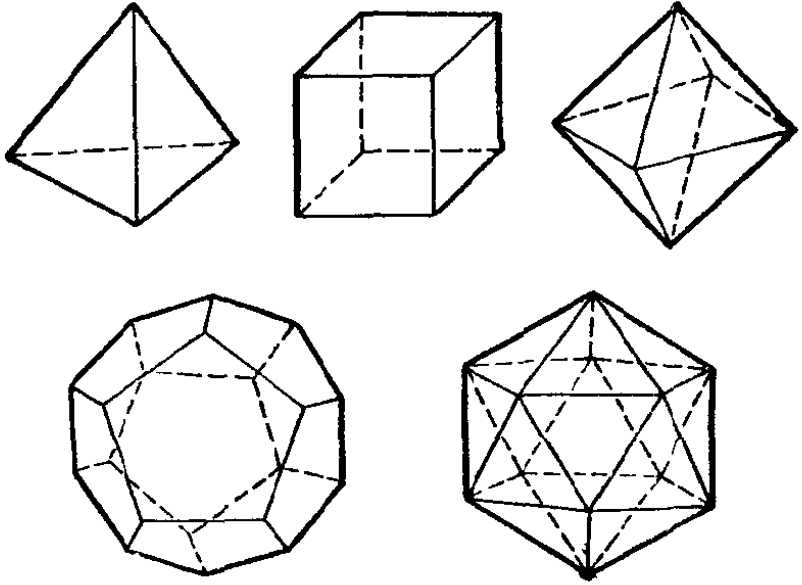
\includegraphics[width=9cm]{../pic/ltjh-ch3-09.png}
    \caption{}\label{fig:ltjh-3-9}
\end{figure}

五种正多面体的表面展开图如图 \ref{fig:ltjh-3-10}。 作为课外研究,可画它 10 倍大的展开图,然后粘成正多面体模型,加以观察。

\begin{figure}[htbp]
    \centering
    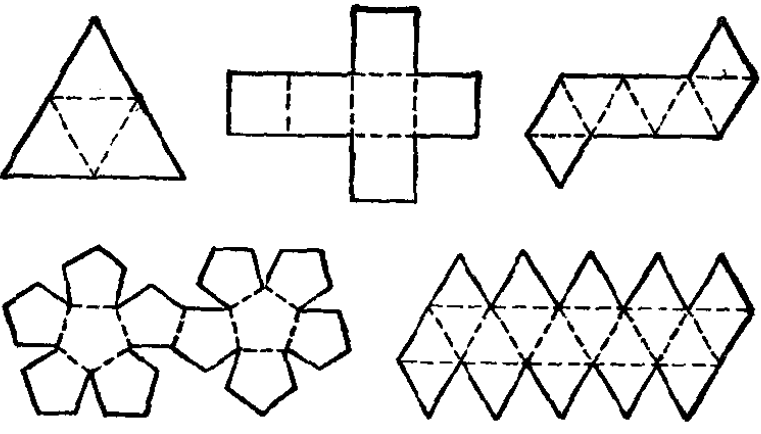
\includegraphics[width=10cm]{../pic/ltjh-ch3-10.png}
    \caption{}\label{fig:ltjh-3-10}
\end{figure}

数一数每种正多面体的顶点数、面数、棱数,分别填在下面表格内,
研究每种正多面体的顶点数、面数与棱数,能否发现它们之间有什么共同关系?

{
\NewExpandableDocumentCommand\fillcolumn{m}{\begin{CJKfilltwosides}{5em}#1\end{CJKfilltwosides}}
\begin{tblr}[expand=\expanded]{hlines, vlines,
    columns={5em,c},
    column{1}={6em},
}
    \fillcolumn{正多面体}   & 顶点数 & 面数 & 棱数 \\
    \fillcolumn{正四面体}   &        &     &      \\
    \fillcolumn{正六面体}   &        &     &      \\
    \fillcolumn{正八面体}   &        &     &      \\
    \fillcolumn{正十二面体} &        &     &      \\
    \fillcolumn{正二十面体} &        &     &      \\
\end{tblr}
}

\begin{lianxi}

\xiaoti{以正多面体的各面中心为顶点的多面体都是几面体?参照模型看它们是不是正多面体?}

\xiaoti{设正十二面体的棱长为 $a$。求它的表面积。}

\end{lianxi}
\end{enhancedline}
